\documentclass[11pt]{article}
\usepackage[utf8]{inputenc}
\usepackage{amsmath,amssymb,booktabs,graphicx,array,xcolor,microtype,threeparttable,caption}
\usepackage[a4paper,margin=1in]{geometry}
\usepackage[numbers,sort&compress]{natbib}
\usepackage[colorlinks=true,linkcolor=blue!50!black,citecolor=blue!50!black,urlcolor=blue!50!black]{hyperref}
\captionsetup{font=small,labelfont=bf}
\usepackage{enumitem}\setlist[itemize]{itemsep=1pt,topsep=2pt}
\newcommand{\todo}[1]{\textcolor{red}{[\textbf{TODO:} #1]}}
\setlength{\parskip}{3pt}
\newcommand{\LLE}{\mathrm{LLE}}
\newcommand{\VPT}{\mathrm{VPT}}
\newcommand{\relnorm}{\|\Delta\theta\|/\|\theta\|}

\title{\textbf{How Much Compression Can a Learned Chaotic Surrogate Survive? A Matched-Control Study of Pruning, Quantization and Attractor Failure in Lorenz-63 and R\"ossler Emulators}}
\author{Viren Singh\\[2pt]\small Independent researcher\\[1pt]\small ORCID: \href{https://orcid.org/0009-0001-6618-0126}{0009-0001-6618-0126}\quad E-mail: \href{mailto:thakurvirensingh1@gmail.com}{thakurvirensingh1@gmail.com}}
\date{Manuscript, October 2026}

\begin{document}
\maketitle

\begin{abstract}
\noindent Neural surrogates of chaotic systems are often compressed by pruning or quantization and judged by a scalar parameter displacement or by one-step error, although they are deployed in long autonomous rollouts. We ask how large a displacement a surrogate survives, whether equal displacement implies equal damage, and whether damage shows up in one-step error first. We train 30 residual MLP surrogates each of Lorenz-63 and R\"ossler and pair every pruning or quantization perturbation with random perturbations of identical total relative norm, plus finer controls (per-tensor norm; pruning support): 21{,}180 perturbed models. Failure dominates (68\% of Lorenz and 79\% of R\"ossler models diverge or collapse), so we use survival-independent endpoints and treat Lyapunov-exponent results as survival-conditional. Half of isotropic perturbations destroy the attractor at a relative displacement of 4.4\% (Lorenz) and 1.8\% (R\"ossler), and 6-bit quantization sits at this radius. At matched total norm, structured perturbations keep valid prediction time longer (17 of 20 comparisons) and have lower one-step error (18 of 20) than isotropic noise, but only 5 of 20 each once per-tensor norms are matched; failure modes also differ. Failure is rarely silent: 98--99\% of failed models already have one-step error at least ten times that of their parent, with a R\"ossler exception. Valid prediction time is log-linear in one-step error ($R^2=0.64$, $0.79$) with a slope that Lyapunov and Jacobian statistics do not explain, and Lyapunov-exponent change is poorly predicted by every quantity tested. Scope: two three-dimensional systems, small MLPs, post-training compression.
\end{abstract}

\noindent\textbf{Keywords:} neural surrogates; chaotic dynamics; model compression; pruning; quantization; Lyapunov exponent; valid prediction time; attractor failure; matched controls

\noindent\textbf{Subject classes:} cs.LG (primary); nlin.CD; physics.comp-ph. MSC 2020: 37M25, 68T07, 37D45.

\medskip
\noindent\fcolorbox{black!40}{black!4}{\parbox{0.96\textwidth}{\small\textbf{Highlights}
\begin{itemize}
\item Half of isotropic weight perturbations destroy a chaotic attractor at 1.8--4.4\% relative norm.
\item Matched-norm controls: structured and random perturbations differ modestly, and in failure mode.
\item Matching per-tensor norms removes most of the advantage over isotropic noise.
\item 98--99\% of failed surrogates already show a tenfold rise in one-step error.
\item Valid prediction time is log-linear in one-step error, with an unexplained slope.
\end{itemize}}}

\section{Introduction}
Neural surrogates are increasingly used as cheap stand-ins for dynamical systems. They are trained to minimise a local, one-step prediction error, but they are often used in closed loop for many steps, where small local errors can be amplified. Recent work analyses this gap between short-time accuracy and long-time consistency directly~\cite{liu2026sns,robertson2026,biswas2026}. Compression adds a second layer of uncertainty: pruning and quantization perturb a trained network in parameter space, and the size of that perturbation is conventionally reported as a sparsity level, a bit width, or a relative weight displacement $\relnorm$. Whether such a scalar says anything reliable about the \emph{dynamical} consequences for a surrogate is not obvious.

This paper started from two hypotheses. H1: compression degrades long-run dynamics before one-step error increases. H2: two perturbations of equal parameter norm can nevertheless have different dynamical effects. A preliminary five-seed pilot suggested support for H2 on the Lorenz system, with the sign of the effect depending on the system. Both hypotheses were stated before the full experiment; we test them in Sections~\ref{sec:h1} and~\ref{sec:matched}. We report here a considerably larger, independently implemented study designed to test these claims more carefully. Its main lesson is methodological: a large share of perturbed chaotic surrogates fail outright, which makes the commonly reported Lyapunov-exponent comparison unreliable unless failures are accounted for.

\paragraph{Contributions.}
\begin{enumerate}
\item A \emph{matched-control protocol}: every structured perturbation is paired with random perturbations of identical total relative norm, identical per-tensor norms, and (for pruning) identical support, so that the roles of magnitude, distribution across layers, and which entries are touched can be separated.
\item Large-scale evidence of how fragile learned chaotic surrogates are to parameter perturbations (failure rates by perturbation type and norm), and a demonstration that conditioning on survival biases LLE-based comparisons.
\item Survival-independent paired comparisons of structured and matched random perturbations (valid prediction time, one-step error, failure), showing a consistent but modest advantage of structured perturbations over isotropic noise that largely disappears once per-tensor norms are matched, and a difference in failure \emph{mode} at matched norm.
\item A direct test of H1 (post hoc): failure rarely occurs while one-step error is still near the parent's (98--99\% of failures already have one-step error at least ten times larger), with a R\"ossler exception; but high one-step error is a non-specific warning, since most survivors exceed this level too.
\item A comparison of predictors of dynamical damage---parameter norm, one-step error, and trajectory-weighted Jacobian-change measures including a first-order Lyapunov-response estimate---with an explicit negative result for predicting LLE change.
\item A \emph{dynamical robustness radius}: the relative displacement at which half of isotropic perturbations destroy the attractor, with bootstrap intervals, which places common compression settings on a single scale.
\item An empirical log-linear relation between one-step error and valid prediction time whose slope is not explained by Lyapunov or Jacobian statistics, and a test of a layer-resolved account of why structured perturbations differ from isotropic noise.
\end{enumerate}

\paragraph{Summary of findings.} Table~\ref{tab:summary} lists the questions and the answers the data give.

\begin{table}[t]
\centering\small
\caption{Research questions and findings. $^\dagger$: exploratory analysis added after the primary results were seen.}\label{tab:summary}
\begin{tabular}{@{}p{0.30\textwidth}p{0.62\textwidth}@{}}
\toprule
Question & Finding\\
\midrule
H1: does failure occur while one-step error is still near the parent's?$^\dagger$ & Rarely: 98--99\% of failed models have at least $10\times$ the parent's one-step error. R\"ossler exception: 16\% of models below $3\times$ fail. High error is sensitive but not specific (\S\ref{sec:h1}).\\[2pt]
H2: does equal norm imply equal dynamics? & Not exactly. Failure modes differ. Structured perturbations beat isotropic noise in 17/20 VPT and 18/20 MSE comparisons, but only 5/20 each against layer-matched noise; LLE comparisons are untestable (\S\ref{sec:matched}).\\[2pt]
How large a displacement does the attractor survive?$^\dagger$ & Half of isotropic perturbations destroy it at 4.4\% (Lorenz) and 1.8\% (R\"ossler) of the parameter norm; 6-bit quantization sits at this radius (\S\ref{sec:radius}).\\[2pt]
Which cheap quantities predict damage? & Parent-relative one-step error predicts VPT loss (CV $R^2$ $0.85$/$0.88$ against $0.77$/$0.74$ for norm); $\Delta$LLE is poorly predicted by all quantities (\S\ref{sec:pred}).\\[2pt]
Why do structured and isotropic perturbations differ?$^\dagger$ & Isotropic noise displaces the output layer $2.5$--$2.8\times$ more at equal total norm; no causal test (\S\ref{sec:mech}).\\
\bottomrule
\end{tabular}
\end{table}

\section{Related Work}
\paragraph{One-step accuracy versus rollout reliability.} Liu, Zanna and Bruna formalise the trade-off between short-time accuracy and long-time consistency in autoregressive surrogates~\cite{liu2026sns}. Robertson et al.\ report that training interventions that improve long-horizon rollout stability of latent surrogate solvers often degrade conventional metrics, including one-step accuracy~\cite{robertson2026}. Biswas compares temporal surrogate architectures on chaotic systems and finds that integrator-like update structure is associated with lower bias and perturbation amplification in rollouts~\cite{biswas2026}. These works concern how surrogates are \emph{trained}; we ask about post-training perturbation of a fixed trained model. Learned chaotic emulators are conventionally scored by valid prediction time in Lyapunov times and by whether they reproduce invariants such as the Lyapunov exponent~\cite{pathak2017,pathak2018,gilpin2023}; our endpoints follow this practice.

\paragraph{Pruning, quantization and dynamics.} Pruning and quantization are standard compression tools~\cite{han2015,jacob2018,hoefler2021}. Pesce et al.\ study magnitude pruning with fine-tuning as a phase transition from a functional to a collapsed regime~\cite{pesce2026}, and Sundaram et al.\ combine component-aware structured pruning with Lyapunov stability criteria for neural controllers~\cite{sundaram2025}. These works motivate evaluating dynamical quantities after compression, but, to our knowledge, do not test whether parameter displacement alone characterises the dynamical effect of a perturbation of a learned chaotic surrogate; our review of the literature is not exhaustive.

\paragraph{Lyapunov exponents.} We use the classical tangent-vector method~\cite{benettin1980,wolf1985} applied to the learned map with analytic Jacobians; the underlying theory is the multiplicative ergodic theorem~\cite{oseledets1968}.

\section{Setup}
\subsection{Systems and surrogates}
We study Lorenz-63~\cite{lorenz1963} ($\sigma=10,\rho=28,\beta=8/3$) and R\"ossler~\cite{rossler1976} ($a=b=0.2,c=5.7$). Trajectories are integrated with fourth-order Runge--Kutta (internal step $10^{-3}$), a $20$ time-unit transient is discarded, and states are sampled every $\Delta t=0.02$. For each seed one trajectory with a random initial condition provides 20{,}000 training transitions and 5{,}000 held-out consecutive test transitions; all states are standardised with training statistics. Reference exponents, computed by tangent-vector integration, are $0.903$ (Lorenz) and $0.0655$ (R\"ossler); we use these values as the Lyapunov time scale.

The surrogate is a residual MLP
\[
f_\theta(x)=x+W_3\tanh\!\big(W_2\tanh(W_1x+b_1)+b_2\big)+b_3,
\]
with two hidden layers of 64 units ($4{,}611$ parameters), trained with Adam~\cite{kingma2015} (learning rate $10^{-3}$, batch 128, 50 epochs) on one-step mean squared error. Training and the Jacobians are implemented in NumPy (manual backpropagation and analytic Jacobians, verified against finite differences). Median test MSE of the 30 Lorenz parents is $4.9\times10^{-6}$ (range $3.3\times10^{-6}$--$3.3\times10^{-5}$) and of the R\"ossler parents $1.5\times10^{-6}$ ($3.2\times10^{-7}$--$1.9\times10^{-5}$) in standardised units.

\subsection{Structured perturbations and matched controls}
The relative displacement of a perturbed model is $\relnorm$ over all parameters, weights and biases. Structured perturbations are: \emph{global} magnitude pruning (smallest weights across all three matrices) and \emph{layer-wise} magnitude pruning at sparsities $25,50,75\%$; post-training per-tensor symmetric uniform quantization at $8,6,4,3$ bits (all tensors); and random (unstructured) pruning at the same sparsities, which has no matched controls and is only reported in aggregate failure rates. Each of the ten global, layer-wise and quantization perturbations is paired with $K=10$ random controls:
\begin{itemize}
\item \textbf{isotropic noise}: Gaussian, rescaled to exactly the same total relative norm;
\item \textbf{layer-matched noise}: Gaussian in each tensor, rescaled to exactly the same per-tensor norm;
\item \textbf{support-matched noise} (pruning only): Gaussian on exactly the entries the pruning altered, with the same per-tensor norms.
\end{itemize}
In addition a calibration cloud of isotropic noise at eight norms ($0.01$--$0.6$, ten draws each) is generated. This gives 353 perturbed models per parent, 21{,}180 in total.

\subsection{Metrics}
\paragraph{Failure.} A rollout \emph{diverges} if it leaves $\|x\|_\infty\le 50$ (standardised units) or becomes non-finite, and \emph{collapses} if it stays bounded but its state standard deviation (mean over coordinates) falls below $0.05$, i.e.\ it settles to a near-constant state. Parents whose own rollout fails or whose LLE estimate is unstable (the two half-run estimates differ by more than $0.25$) are excluded from all analyses: all 30 Lorenz and 22 of 30 R\"ossler parents pass. This leaves $18{,}356$ perturbed models.

\paragraph{One-step error.} Held-out one-step MSE; $|\Delta\mathrm{MSE}|$ is the absolute difference to the parent, and the \emph{ratio} is the perturbed model's MSE divided by its parent's.

\paragraph{Valid prediction time (VPT).} From 20 initial conditions on the test trajectory, the model is rolled out for up to 10 time units; VPT is the first time the normalised error $\|\hat x-x\|/\sqrt{3}$ exceeds $0.4$, averaged over initial conditions and expressed in reference Lyapunov times. It is defined for every model, including failed ones. VPT loss is the parent's VPT minus the perturbed model's. Parent VPT is $1.76\pm0.45$ (Lorenz) and $0.43\pm0.09$ (R\"ossler) Lyapunov times (mean $\pm$ sd).

\paragraph{Largest Lyapunov exponent.} After 1{,}000 transient steps, $10{,}000$ steps (200 time units) of the learned map with analytic Jacobians and tangent-vector renormalisation; defined only for non-failed models whose two half-run estimates agree within $0.25$ (``usable''). The invariant-measure shift is the sliced Wasserstein-1 distance (32 random projections) between 2{,}000 rollout states and test states.

\paragraph{Jacobian-change measures.} Let $\Delta J(x)=J_{\theta'}(x)-J_\theta(x)$ evaluated along the parent's own autonomous orbit (3{,}000 steps; the true orbit if the parent is non-chaotic). We use $S_F=\mathbb{E}\|\Delta J\|_F/\mathbb{E}\|J_\theta\|_F$ and the operator-norm analogue $S_2$. In addition, a signed first-order prediction of $\Delta\LLE$: with the parent's unit tangent vectors $u_t$, $n_t=\|J_tu_t\|$, $v_t=J_tu_t/n_t$,
\[
\log\|(J_t+\Delta J_t)(u_t+\delta u_t)\|\approx\log n_t+\frac{v_t^\top(\Delta J_t u_t+J_t\delta u_t)}{n_t},\quad
\delta u_{t+1}=\frac{(I-v_tv_t^\top)(\Delta J_tu_t+J_t\delta u_t)}{n_t},
\]
and $S_{lin}=\frac{1}{\Delta t}\,\mathbb{E}_t\big[v_t^\top(\Delta J_tu_t+J_t\delta u_t)/n_t\big]$ (and $S_{lin}^{(0)}$ without the direction term $\delta u$). Both are linearisations about a fixed orbit and ignore the shift of the invariant measure.

\subsection{Statistical protocol}\label{sec:stats}
The unit of replication is the parent (seed). For each structured perturbation and control family, we compute per seed the difference between the structured model and the median over the $K$ controls, then report the median over seeds with a 95\% bootstrap interval (4{,}000 resamples), a Wilcoxon signed-rank $p$-value, and Holm-adjusted~\cite{holm1979} $p$-values within each (system, metric) family of 26 tests. Predictors are compared by within-parent Spearman correlation averaged over parents (bootstrap interval over parents) and by a partial Spearman correlation after regressing out the rank of $\relnorm$. The primary analyses (failure rates, matched-pair comparisons and predictor comparison; Sections~\ref{sec:fail}, \ref{sec:matched} and~\ref{sec:pred}) were specified before the full run and not tuned afterwards. All others (the robustness radius, tensor-resolved comparisons, the VPT--MSE relation and the test of H1) were added after the primary results had been seen and are exploratory. The fit window of the VPT--MSE relation was changed after a first version selected on the outcome was found to bias the slope; both versions are reported.

\paragraph{Additional analyses.} The \emph{robustness radius} $r_p$ is obtained by logistic regression of the failure indicator on $\log_{10}\relnorm$ for isotropic-noise perturbations (calibration grid and controls pooled), with 300 bootstrap resamples over parents. The relation between one-step error and VPT is fitted by ordinary least squares of VPT (time units) on $\ln\mathrm{MSE}$ over models with $\log_{10}\mathrm{MSE}\in[-6,-3]$ (a window chosen on the predictor, which does not bias the slope; selecting on low VPT instead truncates the outcome and flattens the slope, and is reported as a sensitivity check), pooled and per parent, and evaluated by leave-one-parent-out $R^2$. Layer-resolved predictors are compared with gradient-boosted regression and classification models (scikit-learn \texttt{HistGradientBoosting}, 200 iterations) under 5-fold cross-validation grouped by parent. The parent's per-tensor relative displacements, and its Jacobian expansion rate $\mathbb{E}[\ln\sigma_{\max}(J)]/\Delta t$ along its own orbit, were obtained by deterministically rebuilding each parent and perturbation set (rebuilds were verified against the stored parent MSE and every model's relative norm).

\section{Results}
\subsection{Most perturbed surrogates fail}\label{sec:fail}
Table~\ref{tab:fail} and Figure~\ref{fig:fail} show that failure is the dominant outcome. Overall, 14\% of Lorenz and 58\% of R\"ossler perturbed models diverge and a further 54\% and 21\% collapse, so only 30\% (Lorenz) and 21\% (R\"ossler) retain a usable LLE. Failure sets in at very small displacements: isotropic noise of relative norm $0.02$ already collapses 37\% of Lorenz surrogates, and 23\% of R\"ossler surrogates diverge at relative norm $0.01$. The R\"ossler parents are themselves only weakly chaotic (mean LLE $0.031\pm0.043$ against a reference of $0.0655$), which probably contributes to their fragility. Because failed models have no LLE, any LLE-based comparison conditions on the mildest perturbations, a selection that becomes severe at larger norms: for global 50\% pruning only 3 Lorenz seeds provide a usable LLE. Random pruning at equal sparsity fails even more often (Lorenz at 50\%: 77\% diverge and 23\% collapse).

\begin{table}[t]
\centering\small
\caption{Fraction of perturbed models that diverge or collapse, by structured perturbation and for isotropic noise of exactly the same norm (valid parents only; 30 Lorenz and 22 R\"ossler parents, 10 noise draws per parent).}\label{tab:fail}
\begin{tabular}{lccccc}
\toprule
 & & \multicolumn{2}{c}{Structured} & \multicolumn{2}{c}{Isotropic noise}\\
\cmidrule(lr){3-4}\cmidrule(lr){5-6}
Perturbation & $\relnorm$ & diverged & collapsed & diverged & collapsed\\
\midrule
\textit{Lorenz-63} (30 valid parents) & & & & & \\
Global pruning 25\% & 0.102 & 0.03 & 0.87 & 0.00 & 0.76 \\
Global pruning 50\% & 0.296 & 0.80 & 0.00 & 0.12 & 0.65 \\
Global pruning 75\% & 0.560 & 0.97 & 0.00 & 0.48 & 0.35 \\
Layer-wise pruning 25\% & 0.108 & 0.00 & 0.63 & 0.00 & 0.73 \\
Layer-wise pruning 50\% & 0.306 & 0.10 & 0.83 & 0.13 & 0.61 \\
Layer-wise pruning 75\% & 0.568 & 0.77 & 0.17 & 0.57 & 0.30 \\
8-bit quantization & 0.009 & 0.00 & 0.07 & 0.00 & 0.10 \\
6-bit quantization & 0.039 & 0.00 & 0.47 & 0.00 & 0.65 \\
4-bit quantization & 0.172 & 0.00 & 0.70 & 0.01 & 0.74 \\
3-bit quantization & 0.402 & 0.07 & 0.67 & 0.27 & 0.55 \\
\midrule
\textit{R\"ossler} (22 valid parents) & & & & & \\
Global pruning 25\% & 0.101 & 0.95 & 0.00 & 0.65 & 0.25 \\
Global pruning 50\% & 0.314 & 0.91 & 0.00 & 0.74 & 0.21 \\
Global pruning 75\% & 0.602 & 0.95 & 0.00 & 0.86 & 0.12 \\
Layer-wise pruning 25\% & 0.117 & 0.27 & 0.18 & 0.56 & 0.30 \\
Layer-wise pruning 50\% & 0.334 & 0.73 & 0.09 & 0.78 & 0.18 \\
Layer-wise pruning 75\% & 0.619 & 1.00 & 0.00 & 0.80 & 0.15 \\
8-bit quantization & 0.007 & 0.09 & 0.00 & 0.18 & 0.05 \\
6-bit quantization & 0.028 & 0.36 & 0.18 & 0.34 & 0.30 \\
4-bit quantization & 0.122 & 0.45 & 0.23 & 0.63 & 0.28 \\
3-bit quantization & 0.286 & 0.86 & 0.09 & 0.74 & 0.20\\
\bottomrule
\end{tabular}
\end{table}

\begin{figure}[t]
\centering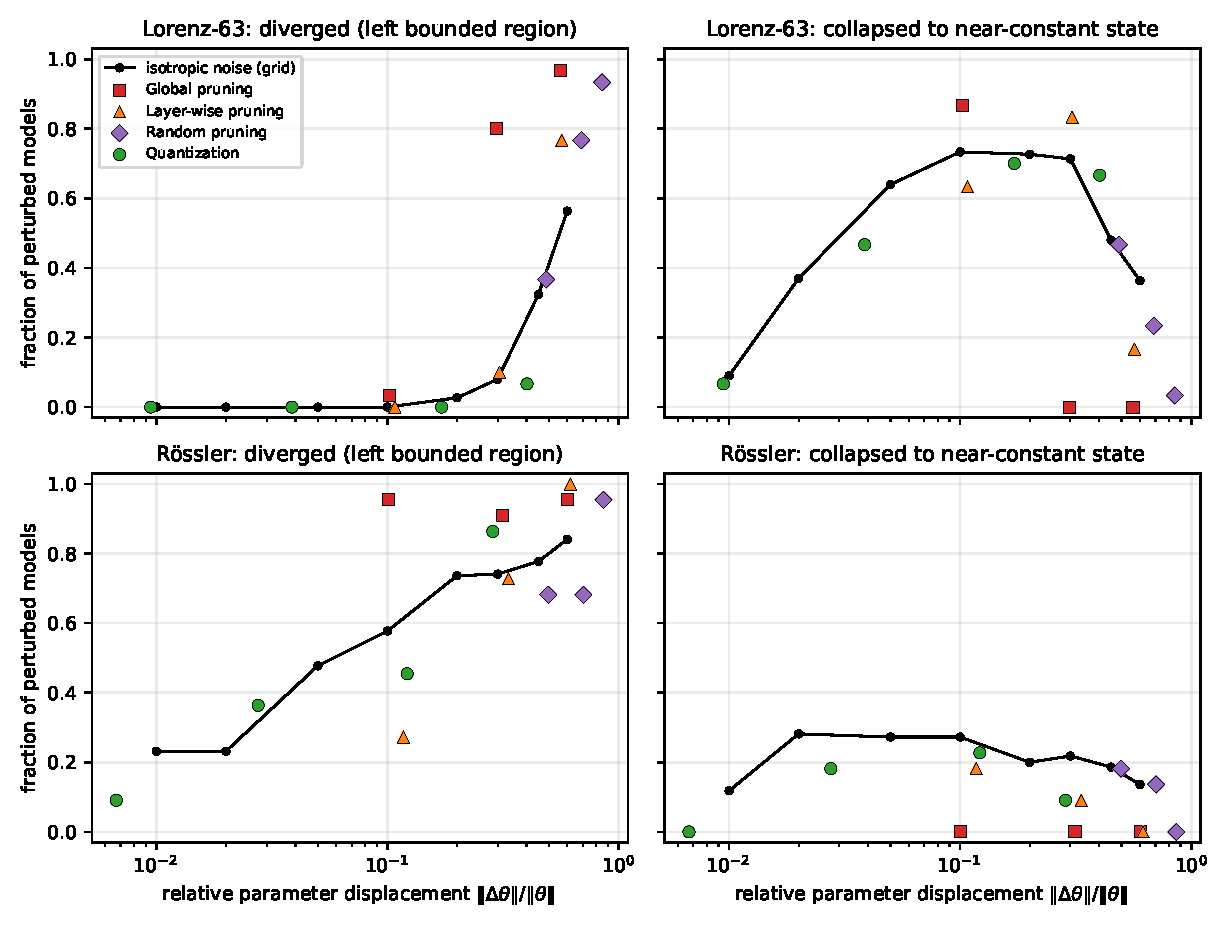
\includegraphics[width=0.92\textwidth]{figures/fig_failure.pdf}
\caption{Failure fractions versus relative displacement. Black: isotropic noise calibration cloud. Markers: structured perturbations. Global magnitude pruning diverges at norms where isotropic noise mostly collapses or survives.}\label{fig:fail}
\end{figure}

\subsection{Dynamical robustness radius}\label{sec:radius}
To place compression settings on one scale we define $r_p$ as the relative displacement at which a fraction $p$ of isotropic-noise perturbations fail (Section~\ref{sec:stats}). Half of isotropic perturbations destroy the attractor at $r_{50}=0.044$ [0.038, 0.051] of the parameter norm for Lorenz and $0.018$ [0.015, 0.021] for R\"ossler (Table~\ref{tab:radius}, Figure~\ref{fig:radius}); the 10\% radius is only about $0.2$--$0.3\%$ for both. Divergence alone is rarer ($r_{50}^{\mathrm{div}}=0.55$ and $0.064$) because isotropic noise on Lorenz mostly collapses the attractor to a fixed point rather than blowing it up. Structured perturbations fall on a similar scale: 8-bit quantization (relative norm $0.009$ and $0.007$) fails in 7\% and 9\% of models, 6-bit ($0.039$, $0.028$) in 47\% and 55\%, i.e.\ at the radius, and 25\% global or layer-wise pruning (relative norm about $0.10$) already fails in 90\% and 63\% of Lorenz and 95\% and 45\% of R\"ossler models. The radius is conditional on the collapse threshold (state standard deviation $0.05$), the logistic form, and this architecture and training recipe.

\begin{table}[t]
\centering\small
\caption{Dynamical robustness radius $r_p$: relative displacement at which a fraction $p$ of isotropic-noise perturbations fail (95\% bootstrap intervals over parents). Last column: radius for divergence only ($p=0.5$).}\label{tab:radius}
\begin{tabular}{lcccc}
\toprule
System & $r_{10}$ & $r_{50}$ & $r_{90}$ & $r_{50}$ (diverge only)\\
\midrule
Lorenz-63 & 0.0028 [0.002, 0.0038] & 0.044 [0.038, 0.05] & 0.7 [0.61, 0.84] & 0.55 [0.53, 0.56] \\
R\"ossler & 0.0023 [0.0017, 0.003] & 0.018 [0.015, 0.021] & 0.14 [0.13, 0.16] & 0.064 [0.052, 0.076]\\
\bottomrule
\end{tabular}
\end{table}

\begin{figure}[t]
\centering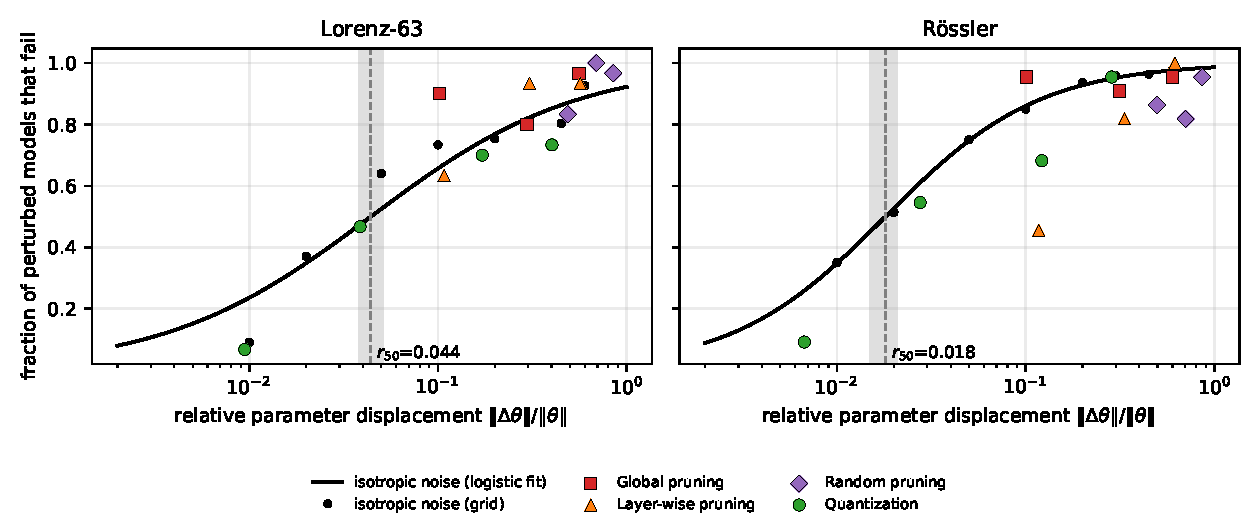
\includegraphics[width=0.95\textwidth]{figures/fig_robustness.pdf}
\caption{Failure fraction versus relative displacement. Black: isotropic noise with logistic fit; gray band: 95\% interval of $r_{50}$. Markers: structured perturbations.}\label{fig:radius}
\end{figure}

\subsection{Does failure appear before one-step error rises?}\label{sec:h1}
Hypothesis H1 says compression degrades long-run dynamics while one-step error is still near the parent's. We tested it post hoc by binning every perturbed model of a valid parent by its ratio (perturbed MSE over parent MSE) and tabulating failure (Table~\ref{tab:h1}, Figure~\ref{fig:h1}). Failure is uncommon at small ratios and rises steeply with the ratio on both systems: on Lorenz, 6\% of models with a ratio below 3 fail, against 25\% at 10--30 and 80\% above 1000. Failures are concentrated at large ratios: 99.1\% (Lorenz) and 98.0\% (R\"ossler) of failed models have a ratio of at least 10, and only 0.2\% and 0.6\% have a ratio below 3. In this sense failure is rarely silent. The converse does not hold: 79\% (Lorenz) and 72\% (R\"ossler) of surviving models also have a ratio of at least 10, so a tenfold rise in one-step error is a sensitive but non-specific warning.

R\"ossler is a partial exception: 16\% [6, 28] of models with a ratio below 3 fail, almost all by divergence. These 37 models come from 10 of the 22 valid parents; all but one are random-noise models, at the norm of 8-bit quantization ($\approx0.007$; 28 models), of 6-bit quantization (two models) or the smallest calibration norm ($0.01$; six models), and the one structured case is an 8-bit-quantized model. On Lorenz the corresponding 18 models come from 7 of 30 parents (again one structured case, 8-bit quantization). The R\"ossler parents are weakly chaotic (mean exponent $0.031$), which would be consistent with some of them sitting close to a stability boundary, but we did not test this. Because the design samples a few fixed norms rather than a continuous compression path, the analysis is cross-sectional: it shows how failure co-occurs with one-step error, not the order in which they appear along a path.

\begin{table}[t]
\centering\small
\caption{Failure by parent-relative one-step error (ratio = perturbed MSE / parent MSE; valid parents only). Failed: diverged or collapsed, with 95\% bootstrap interval over parents; ``div.'': percentage that diverged.}\label{tab:h1}
\begin{tabular}{lcccccc}
\toprule
 & \multicolumn{3}{c}{Lorenz-63} & \multicolumn{3}{c}{R\"ossler}\\
\cmidrule(lr){2-4}\cmidrule(lr){5-7}
Ratio & models & failed (\%) & div. (\%) & models & failed (\%) & div. (\%)\\
\midrule
$<$3 & 298 & 6 [2, 11] & 0 & 237 & 16 [6, 28] & 15 \\
3--10 & 482 & 9 [4, 15] & 0 & 338 & 26 [19, 32] & 19 \\
10--30 & 525 & 25 [20, 32] & 0 & 393 & 42 [35, 49] & 24 \\
30--100 & 593 & 54 [48, 61] & 0 & 512 & 55 [48, 62] & 31 \\
100--1000 & 2{,}274 & 69 [66, 72] & 1 & 1{,}652 & 77 [71, 81] & 50 \\
$>$1000 & 6{,}418 & 80 [79, 81] & 23 & 4{,}634 & 93 [92, 94] & 72\\
\bottomrule
\end{tabular}
\end{table}

\begin{figure}[t]
\centering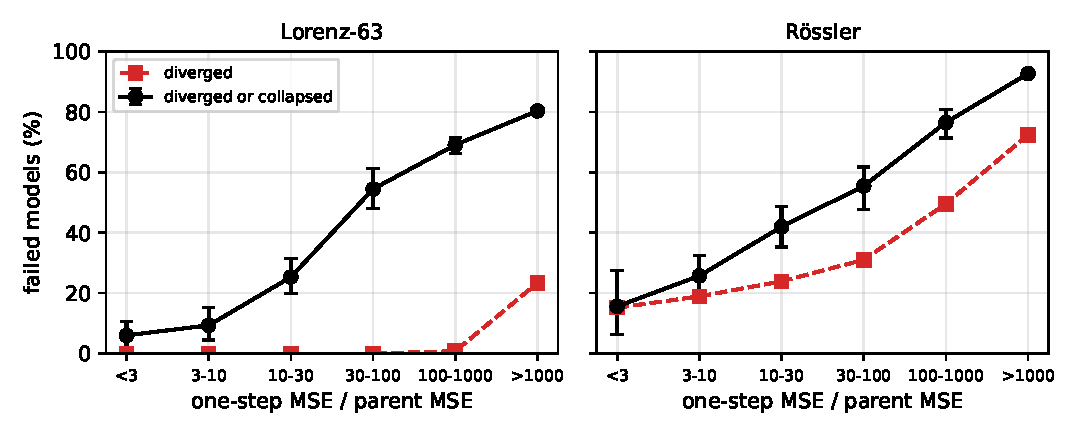
\includegraphics[width=0.92\textwidth]{figures/fig_h1.pdf}
\caption{Fraction of perturbed models that fail, by parent-relative one-step error (bars: 95\% bootstrap interval over parents). Red dashed: divergence only.}\label{fig:h1}
\end{figure}

\subsection{Matched-norm perturbations are not equivalent, but the differences are modest}\label{sec:matched}
Figure~\ref{fig:forest} and Tables~\ref{tab:vpt} and~\ref{tab:mse} compare each structured perturbation with its controls using survival-independent endpoints on all 30 (Lorenz) or 22 (R\"ossler) seeds.

\paragraph{Versus isotropic noise.} Structured perturbations have significantly longer VPT than norm-matched isotropic noise in 17 of 20 comparisons and significantly shorter in one (Lorenz global 25\%); two are not significant. One-step error is significantly lower in 18 of 20 comparisons and higher in one (the same case). The direction is therefore the same on both systems. In absolute terms, VPT differences are small: median differences range from $-0.03$ to $+0.32$ Lyapunov times on Lorenz (parent VPT $1.76$) and up to $+0.10$ on R\"ossler (parent $0.43$). One-step errors differ by up to a factor of about 5 (Lorenz, $\log_{10}$ difference $-0.69$) and 39 (R\"ossler, $-1.59$).

\paragraph{Versus finer controls.} Matching per-tensor norms removes most of the difference: only 5 of 20 VPT comparisons and 5 of 20 MSE comparisons remain significant (VPT in favour of the structured perturbation in all 5; MSE lower in 4 and higher in 1). For pruning, matching the support as well leaves 4 of 12 VPT and 6 of 12 MSE comparisons significant, again with small VPT effects ($0.011$--$0.022$ Lyapunov times). This suggests that much of the advantage over isotropic noise reflects how the displacement is spread across tensors rather than which individual entries or values are altered; Section~\ref{sec:mech} examines which tensors are involved.

\paragraph{Failure rates and failure modes.} Total failure rates at matched norm are often similar, but the mode differs (Table~\ref{tab:fail}). Global 50\% magnitude pruning fails in 80\% of Lorenz parents, all by divergence, while isotropic noise of the same norm fails in 77\%, mostly by collapse (65\%) and diverges only 12\%; at 75\%, 97\% against 48\% diverge. Quantization behaves the other way: at 3 bits 7\% diverge versus 27\% for noise. On R\"ossler, global pruning diverges in 91--96\% of seeds at every sparsity level.

\paragraph{LLE.} Among the 14 (structured, control) pairs with at least six usable seeds, none reaches $p<0.05$ and the structured model sits at a mean percentile of $0.36$--$0.67$ of its control distribution. These pairs are almost all 8-, 6- or 4-bit quantization or 25\% layer-wise pruning, i.e.\ the mildest perturbations; for larger perturbations only 1--3 seeds are usable and no test can be made. The sign pattern reported in the preliminary pilot (pruning more contracting than matched noise on Lorenz at 50\%) could not be assessed for this reason.

\begin{figure}[t]
\centering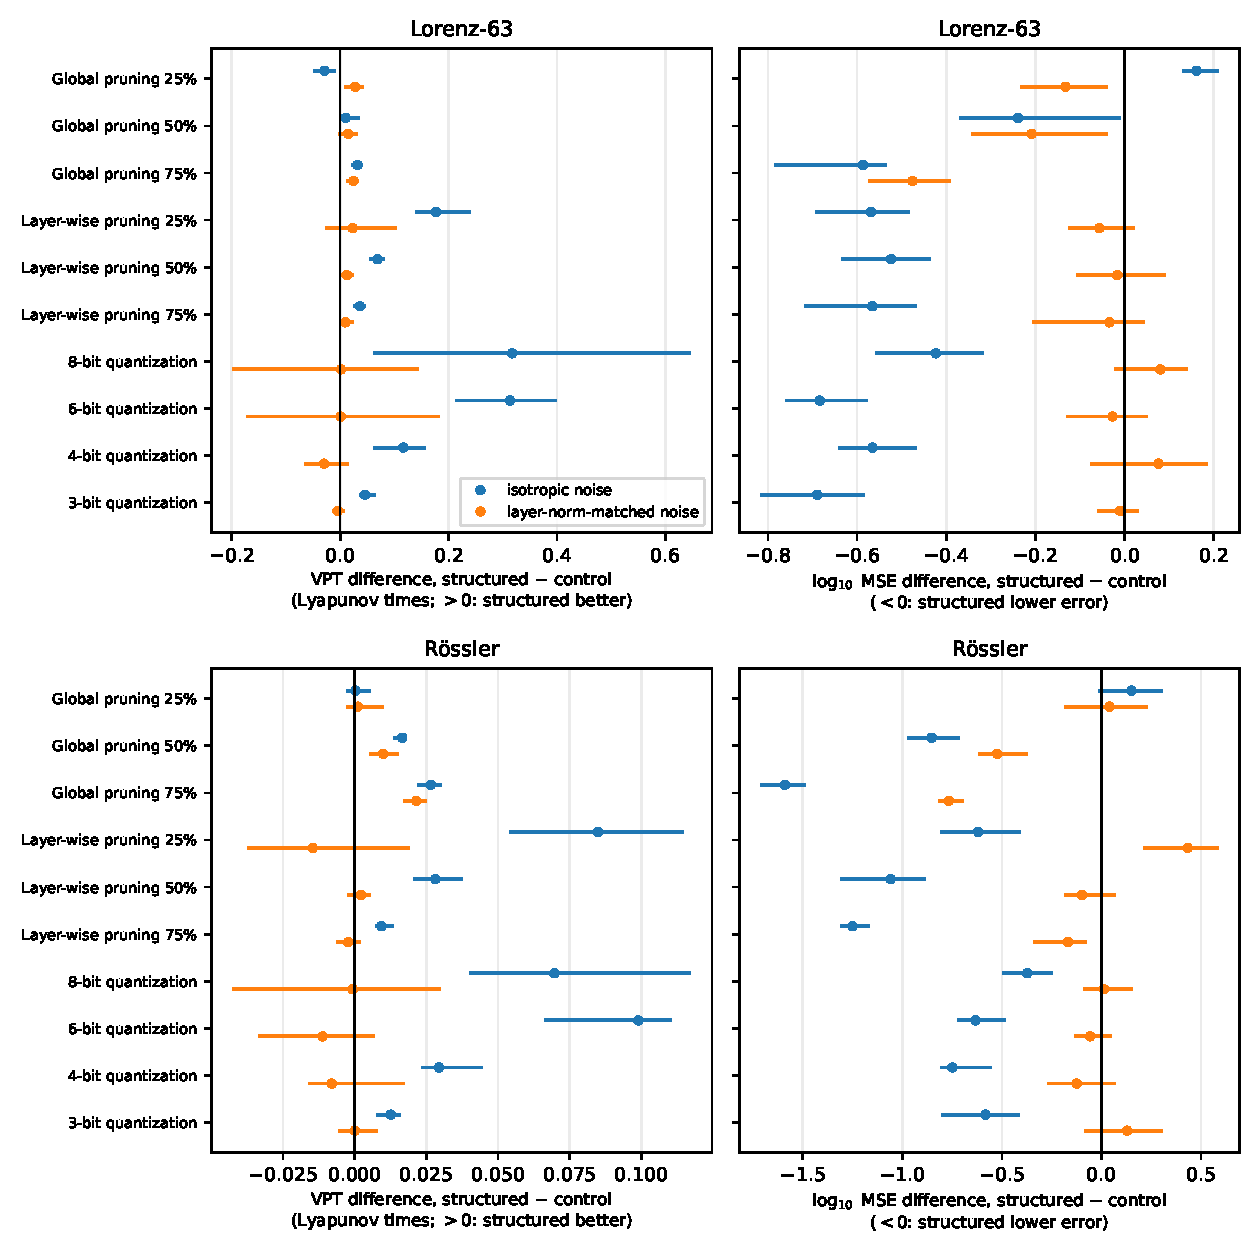
\includegraphics[width=0.95\textwidth]{figures/fig_forest.pdf}
\caption{Paired differences between each structured perturbation and its norm-matched controls (median over seeds, 95\% bootstrap interval). Left: valid prediction time (positive: structured better). Right: $\log_{10}$ one-step MSE (negative: structured better).}\label{fig:forest}
\end{figure}

\begin{table}[t]
\centering\scriptsize
\caption{Valid prediction time difference, structured $-$ control (Lyapunov times; median over seeds, 95\% bootstrap interval; Holm-adjusted $p$). Positive: structured model predicts longer.}\label{tab:vpt}
\resizebox{\textwidth}{!}{%
\begin{tabular}{lcccccc}
\toprule
 & & & \multicolumn{2}{c}{vs isotropic noise} & \multicolumn{2}{c}{vs layer-matched noise}\\
\cmidrule(lr){4-5}\cmidrule(lr){6-7}
Structured & $\relnorm$ & seeds & difference & $p_{\mathrm{Holm}}$ & difference & $p_{\mathrm{Holm}}$\\
\midrule
\textit{Lorenz-63} & & & & & \\
Global pruning 25\% & 0.102 & 30 & -0.029 [-0.047, -0.011] & $<$0.001 & +0.028 [+0.010, +0.040] & $<$0.001 \\
Global pruning 50\% & 0.296 & 30 & +0.010 [+0.001, +0.033] & 0.057 & +0.015 [-0.000, +0.029] & 0.056 \\
Global pruning 75\% & 0.560 & 30 & +0.032 [+0.023, +0.038] & $<$0.001 & +0.024 [+0.015, +0.030] & $<$0.001 \\
Layer-wise pruning 25\% & 0.108 & 30 & +0.177 [+0.141, +0.237] & $<$0.001 & +0.023 [-0.025, +0.102] & 0.803 \\
Layer-wise pruning 50\% & 0.306 & 30 & +0.069 [+0.057, +0.080] & $<$0.001 & +0.012 [+0.004, +0.022] & 0.453 \\
Layer-wise pruning 75\% & 0.568 & 30 & +0.036 [+0.028, +0.044] & $<$0.001 & +0.009 [+0.003, +0.022] & 0.042 \\
8-bit quantization & 0.009 & 30 & +0.317 [+0.065, +0.644] & 0.006 & +0.002 [-0.196, +0.141] & 1.000 \\
6-bit quantization & 0.039 & 30 & +0.313 [+0.216, +0.396] & $<$0.001 & +0.001 [-0.170, +0.180] & 1.000 \\
4-bit quantization & 0.172 & 30 & +0.117 [+0.064, +0.155] & $<$0.001 & -0.030 [-0.063, +0.012] & 1.000 \\
3-bit quantization & 0.402 & 30 & +0.046 [+0.038, +0.063] & $<$0.001 & -0.004 [-0.012, +0.005] & 1.000 \\
\midrule
\textit{R\"ossler} & & & & & \\
Global pruning 25\% & 0.101 & 22 & +0.000 [-0.002, +0.005] & 1.000 & +0.001 [-0.002, +0.010] & 1.000 \\
Global pruning 50\% & 0.314 & 22 & +0.017 [+0.014, +0.017] & $<$0.001 & +0.010 [+0.006, +0.015] & $<$0.001 \\
Global pruning 75\% & 0.602 & 22 & +0.027 [+0.023, +0.030] & $<$0.001 & +0.022 [+0.018, +0.025] & $<$0.001 \\
Layer-wise pruning 25\% & 0.117 & 22 & +0.085 [+0.055, +0.114] & $<$0.001 & -0.015 [-0.037, +0.019] & 1.000 \\
Layer-wise pruning 50\% & 0.334 & 22 & +0.028 [+0.021, +0.037] & $<$0.001 & +0.002 [-0.002, +0.005] & 1.000 \\
Layer-wise pruning 75\% & 0.619 & 22 & +0.009 [+0.008, +0.013] & $<$0.001 & -0.002 [-0.006, +0.002] & 1.000 \\
8-bit quantization & 0.007 & 22 & +0.070 [+0.041, +0.117] & $<$0.001 & -0.001 [-0.042, +0.029] & 1.000 \\
6-bit quantization & 0.028 & 22 & +0.099 [+0.067, +0.110] & $<$0.001 & -0.011 [-0.033, +0.006] & 1.000 \\
4-bit quantization & 0.122 & 22 & +0.029 [+0.024, +0.044] & $<$0.001 & -0.008 [-0.016, +0.017] & 1.000 \\
3-bit quantization & 0.286 & 22 & +0.013 [+0.008, +0.016] & $<$0.001 & +0.000 [-0.005, +0.007] & 1.000\\
\bottomrule
\end{tabular}}
\end{table}

\begin{table}[t]
\centering\scriptsize
\caption{$\log_{10}$ one-step MSE difference, structured $-$ control. Negative: structured model has lower error.}\label{tab:mse}
\resizebox{\textwidth}{!}{%
\begin{tabular}{lcccccc}
\toprule
 & & & \multicolumn{2}{c}{vs isotropic noise} & \multicolumn{2}{c}{vs layer-matched noise}\\
\cmidrule(lr){4-5}\cmidrule(lr){6-7}
Structured & $\relnorm$ & seeds & difference & $p_{\mathrm{Holm}}$ & difference & $p_{\mathrm{Holm}}$\\
\midrule
\textit{Lorenz-63} & & & & & \\
Global pruning 25\% & 0.102 & 30 & +0.16 [+0.13, +0.21] & 0.001 & -0.13 [-0.23, -0.04] & 0.001 \\
Global pruning 50\% & 0.296 & 30 & -0.24 [-0.37, -0.01] & 0.036 & -0.21 [-0.34, -0.04] & 0.065 \\
Global pruning 75\% & 0.560 & 30 & -0.59 [-0.78, -0.54] & $<$0.001 & -0.48 [-0.57, -0.39] & $<$0.001 \\
Layer-wise pruning 25\% & 0.108 & 30 & -0.57 [-0.69, -0.49] & $<$0.001 & -0.06 [-0.12, +0.02] & 1.000 \\
Layer-wise pruning 50\% & 0.306 & 30 & -0.52 [-0.63, -0.44] & $<$0.001 & -0.02 [-0.10, +0.09] & 1.000 \\
Layer-wise pruning 75\% & 0.568 & 30 & -0.57 [-0.71, -0.47] & $<$0.001 & -0.03 [-0.20, +0.04] & 0.757 \\
8-bit quantization & 0.009 & 30 & -0.42 [-0.56, -0.32] & $<$0.001 & +0.08 [-0.02, +0.14] & 0.494 \\
6-bit quantization & 0.039 & 30 & -0.68 [-0.76, -0.58] & $<$0.001 & -0.03 [-0.13, +0.05] & 1.000 \\
4-bit quantization & 0.172 & 30 & -0.57 [-0.64, -0.47] & $<$0.001 & +0.08 [-0.07, +0.18] & 1.000 \\
3-bit quantization & 0.402 & 30 & -0.69 [-0.81, -0.59] & $<$0.001 & -0.01 [-0.06, +0.03] & 1.000 \\
\midrule
\textit{R\"ossler} & & & & & \\
Global pruning 25\% & 0.101 & 22 & +0.15 [-0.01, +0.30] & 0.949 & +0.04 [-0.18, +0.22] & 1.000 \\
Global pruning 50\% & 0.314 & 22 & -0.85 [-0.97, -0.72] & $<$0.001 & -0.52 [-0.61, -0.38] & $<$0.001 \\
Global pruning 75\% & 0.602 & 22 & -1.59 [-1.70, -1.49] & $<$0.001 & -0.77 [-0.81, -0.70] & $<$0.001 \\
Layer-wise pruning 25\% & 0.117 & 22 & -0.62 [-0.80, -0.42] & $<$0.001 & +0.43 [+0.22, +0.58] & 0.005 \\
Layer-wise pruning 50\% & 0.334 & 22 & -1.06 [-1.30, -0.89] & $<$0.001 & -0.10 [-0.18, +0.06] & 1.000 \\
Layer-wise pruning 75\% & 0.619 & 22 & -1.25 [-1.30, -1.17] & $<$0.001 & -0.17 [-0.33, -0.08] & 0.156 \\
8-bit quantization & 0.007 & 22 & -0.37 [-0.49, -0.25] & $<$0.001 & +0.01 [-0.08, +0.15] & 1.000 \\
6-bit quantization & 0.028 & 22 & -0.63 [-0.72, -0.49] & $<$0.001 & -0.06 [-0.13, +0.04] & 1.000 \\
4-bit quantization & 0.122 & 22 & -0.75 [-0.80, -0.56] & $<$0.001 & -0.12 [-0.26, +0.06] & 1.000 \\
3-bit quantization & 0.286 & 22 & -0.58 [-0.80, -0.42] & $<$0.001 & +0.13 [-0.08, +0.30] & 1.000\\
\bottomrule
\end{tabular}}
\end{table}

\subsection{Which tensors carry the difference?}\label{sec:mech}
All families put 89--97\% of the squared displacement into the large middle matrix $W_2$ (4{,}096 of 4{,}611 parameters; Table~\ref{tab:shares}), so the total-norm match hides little there. The difference is in the small output layer $W_3$ and the biases: at matched total norm, isotropic noise displaces $W_3$ in relative terms $2.8\times$ (Lorenz) and $2.5\times$ (R\"ossler) more than the structured perturbations it is paired with (median over the ten structured groups), whereas $W_1$ and $W_2$ are displaced about equally (ratios $0.8$--$1.1$). The output layer is small by initialisation and directly sets the residual step, which is consistent with layer-matched noise removing most of the advantage; we did not isolate it causally, for example by perturbing $W_3$ alone.

Table~\ref{tab:cv} gives a coarse predictive check. Adding the perturbation family to the scalar norm does not change the cross-validated $R^2$ of VPT loss ($0.766\to0.767$ on Lorenz, $0.738\to0.739$ on R\"ossler) or the failure AUC, and neither does adding it to the per-tensor displacements. This is weak evidence on the mechanism: structured perturbations are only 13 of the 353 models per parent, so a flexible model has little to learn from the family indicator, and it also indicates that family adds nothing beyond what the scalar norm already encodes at this resolution. Replacing the scalar norm by the six per-tensor displacements raises $R^2$ from $0.77$ to $0.79$ (Lorenz) and from $0.74$ to $0.82$ (R\"ossler), so how the displacement is distributed across tensors carries some information on R\"ossler and little on Lorenz. The largest gain comes from the parent-relative one-step error: $R^2$ rises to $0.85$ and $0.88$, i.e.\ about 36\% and 55\% of the variance left unexplained by norm, and the full model reaches $0.86$ and $0.90$. The failure AUC is not improved by one-step error.

\begin{table}[t]
\centering\small
\caption{Share (\%) of squared displacement per tensor group (mean over models of valid parents).}\label{tab:shares}
\begin{tabular}{lcccc}
\toprule
 & $W_1$ & $W_2$ & $W_3$ & biases\\
\midrule
\textit{Lorenz-63} & & & & \\
Isotropic noise & 4.2 & 88.8 & 4.2 & 2.8 \\
Layer-matched noise & 3.4 & 94.2 & 2.0 & 0.3 \\
Global pruning & 3.7 & 90.9 & 5.4 & 0.0 \\
Layer-wise pruning & 5.7 & 93.8 & 0.6 & 0.0 \\
Quantization & 1.6 & 97.0 & 0.6 & 0.8 \\
\textit{R\"ossler} & & & & \\
Isotropic noise & 4.2 & 88.8 & 4.2 & 2.9 \\
Layer-matched noise & 5.6 & 93.0 & 1.2 & 0.2 \\
Global pruning & 3.3 & 93.8 & 2.9 & 0.0 \\
Layer-wise pruning & 6.5 & 93.5 & 0.0 & 0.0 \\
Quantization & 6.7 & 92.1 & 0.8 & 0.5\\
\bottomrule
\end{tabular}
\end{table}

\begin{table}[t]
\centering\small
\caption{Cross-validated (5 folds grouped by parent) gradient-boosted models: $R^2$ for the fraction of VPT lost and AUC for failure. ``Relative MSE'' is the perturbed model's one-step MSE divided by the parent's. Family is the perturbation type.}\label{tab:cv}
\begin{tabular}{lcccc}
\toprule
 & \multicolumn{2}{c}{Lorenz-63} & \multicolumn{2}{c}{R\"ossler}\\
\cmidrule(lr){2-3}\cmidrule(lr){4-5}
Features & $R^2$ & AUC & $R^2$ & AUC\\
\midrule
scalar norm & 0.766 & 0.713 & 0.738 & 0.805 \\
scalar norm + family & 0.767 & 0.714 & 0.739 & 0.804 \\
per-tensor norms & 0.787 & 0.716 & 0.818 & 0.816 \\
per-tensor norms + family & 0.788 & 0.716 & 0.817 & 0.816 \\
scalar norm + relative MSE & 0.851 & 0.707 & 0.881 & 0.801 \\
per-tensor + family + relative MSE & 0.859 & 0.713 & 0.896 & 0.815\\
\bottomrule
\end{tabular}
\end{table}

\subsection{What predicts dynamical damage?}\label{sec:pred}
Figure~\ref{fig:pred} and Table~\ref{tab:pred} give within-parent rank correlations between candidate predictors and three damage measures. VPT loss is computed over all perturbed models of valid parents ($10{,}590$ Lorenz, $7{,}766$ R\"ossler); LLE change and invariant-measure shift are only defined for non-failed models and are computed over usable models ($3{,}208$ and $1{,}634$).

\begin{table}[t]
\centering\small
\caption{Within-parent Spearman $\rho$ (mean over parents; 95\% bootstrap interval over parents) between each predictor and each damage measure. VPT loss uses all perturbed models; the other two use usable (non-failed) models only.}\label{tab:pred}
\begin{tabular}{lccc}
\toprule
Predictor & $|\Delta\LLE|$ & VPT loss & SW$_1$ shift\\
\midrule
\textit{Lorenz-63} & & & \\
$\|\Delta\theta\|/\|\theta\|$ & 0.61 [0.53, 0.67] & 0.84 [0.84, 0.85] & 0.76 [0.73, 0.78] \\
$S_F$ (relative) & 0.64 [0.54, 0.70] & 0.90 [0.90, 0.91] & 0.79 [0.77, 0.80] \\
$S_2$ & 0.64 [0.54, 0.70] & 0.90 [0.90, 0.91] & 0.79 [0.77, 0.80] \\
$|S_{lin}|$ & 0.54 [0.46, 0.60] & 0.69 [0.68, 0.70] & 0.66 [0.63, 0.68] \\
$|S_{lin}^{(0)}|$ & 0.53 [0.45, 0.58] & 0.70 [0.68, 0.71] & 0.66 [0.63, 0.68] \\
$|\Delta$ one-step MSE$|$ & 0.65 [0.55, 0.71] & 0.98 [0.98, 0.98] & 0.81 [0.79, 0.82] \\
\midrule
\textit{R\"ossler} & & & \\
$\|\Delta\theta\|/\|\theta\|$ & 0.08 [-0.01, 0.17] & 0.74 [0.73, 0.75] & 0.61 [0.53, 0.68] \\
$S_F$ (relative) & 0.09 [-0.01, 0.18] & 0.93 [0.91, 0.95] & 0.68 [0.59, 0.74] \\
$S_2$ & 0.09 [-0.00, 0.18] & 0.93 [0.90, 0.94] & 0.68 [0.59, 0.74] \\
$|S_{lin}|$ & 0.10 [0.02, 0.18] & 0.75 [0.74, 0.77] & 0.59 [0.53, 0.63] \\
$|S_{lin}^{(0)}|$ & 0.07 [-0.01, 0.16] & 0.74 [0.72, 0.76] & 0.59 [0.51, 0.65] \\
$|\Delta$ one-step MSE$|$ & 0.07 [-0.02, 0.17] & 0.95 [0.95, 0.96] & 0.69 [0.61, 0.74]\\
\bottomrule
\end{tabular}
\end{table}

\begin{figure}[t]
\centering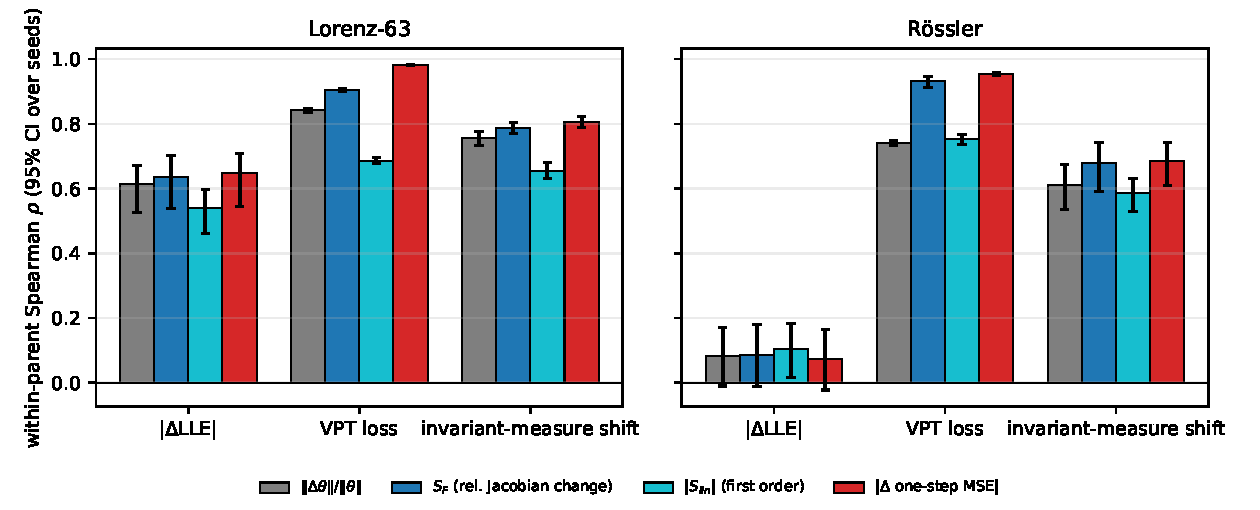
\includegraphics[width=0.92\textwidth]{figures/fig_predictivity.pdf}
\caption{Within-parent Spearman correlation of predictors with damage measures (bars: 95\% bootstrap interval over parents).}\label{fig:pred}
\end{figure}

\begin{figure}[t]
\centering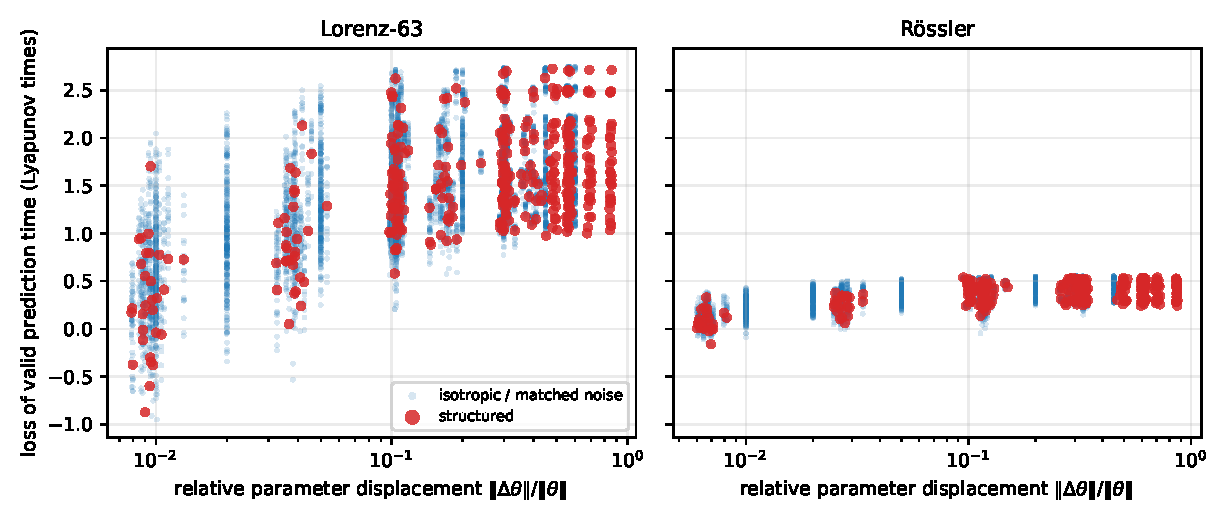
\includegraphics[width=0.95\textwidth]{figures/fig_vpt_vs_norm.pdf}
\caption{Loss of valid prediction time versus relative displacement for structured perturbations (red) and random controls (blue). At a given norm, VPT loss spans a wide range.}\label{fig:vpt}
\end{figure}

\paragraph{Parameter norm orders damage across scales but not at fixed norm.} Relative norm has within-parent $\rho=0.84$ (Lorenz) and $0.74$ (R\"ossler) with VPT loss, which mostly reflects that damage grows with perturbation size over two orders of magnitude (Figure~\ref{fig:vpt}). At fixed norm the information it carries vanishes by construction, and what remains varies widely across perturbations (Figure~\ref{fig:vpt}).

\paragraph{One-step error is the strongest predictor of VPT loss.} In rank terms $|\Delta\mathrm{MSE}|$ attains $\rho=0.98$ (Lorenz) and $0.95$ (R\"ossler) with VPT loss, and its partial correlation given norm is $0.94$ and $0.90$ (Table~\ref{tab:partial}), versus $0.61$ and $0.85$ for the Jacobian-change measure $S_F$ and $0.16$ and $0.53$ for the first-order $|S_{lin}|$. In variance terms the gain is smaller (Section~\ref{sec:mech}: parent-relative one-step error explains 36\% and 55\% of the variance that norm leaves unexplained). This is expected in part: VPT is a short-horizon quantity (at most 10 time units here) and measures accumulated one-step error amplified by local expansion, so it is not independent of one-step error. We read the result as showing that, for post-training perturbation of a fixed surrogate, one-step error computed on the same distribution is a strong predictor of how long the rollout stays accurate, in contrast to what is reported for training interventions~\cite{robertson2026}.

\paragraph{LLE change is poorly predicted by everything.} On Lorenz, correlations with $|\Delta\LLE|$ are $\rho=0.61$--$0.65$ for norm, $S_F$ and one-step error, with partial correlations given norm of only $0.24$ ($S_F$) and $0.29$ (MSE); on R\"ossler all predictors are at $\rho\le0.11$ with intervals that include or nearly include zero. Long-run exponent damage is thus not captured by norm, one-step error, or Jacobian change, at least within the usable subset. The signed prediction $S_{lin}$ has sign agreement with measured $\Delta\LLE$ of $0.54$ (Lorenz) and $0.58$ (R\"ossler), close to chance, even for relative norm $\le0.1$ ($0.52$ and $0.60$).

\paragraph{Predicting failure.} For divergence or collapse, AUCs are $0.73$--$0.74$ (Lorenz) and $0.79$--$0.84$ (R\"ossler) for norm, $S_F$ and one-step error, with the Jacobian and MSE measures marginally above norm (Table~\ref{tab:auc}).

\begin{table}[t]
\centering\small
\begin{minipage}[t]{0.48\textwidth}\centering
\caption{Partial Spearman $\rho$ given $\relnorm$ (mean over parents).}\label{tab:partial}
\begin{tabular}{lccc}
\toprule
Predictor & $|\Delta\LLE|$ & VPT loss & SW$_1$\\
\midrule
\textit{Lorenz-63} & & & \\
$\|\Delta\theta\|/\|\theta\|$ & 0.00 & -0.01 & 0.00 \\
$S_F$ (relative) & 0.24 & 0.61 & 0.34 \\
$S_2$ & 0.24 & 0.60 & 0.34 \\
$|S_{lin}|$ & 0.11 & 0.16 & 0.13 \\
$|S_{lin}^{(0)}|$ & 0.07 & 0.22 & 0.12 \\
$|\Delta$ one-step MSE$|$ & 0.29 & 0.93 & 0.43 \\
\midrule
\textit{R\"ossler} & & & \\
$\|\Delta\theta\|/\|\theta\|$ & 0.00 & 0.01 & -0.03 \\
$S_F$ (relative) & 0.03 & 0.85 & 0.40 \\
$S_2$ & 0.03 & 0.83 & 0.39 \\
$|S_{lin}|$ & 0.07 & 0.53 & 0.25 \\
$|S_{lin}^{(0)}|$ & 0.03 & 0.56 & 0.29 \\
$|\Delta$ one-step MSE$|$ & 0.00 & 0.90 & 0.41\\
\bottomrule
\end{tabular}
\end{minipage}\hfill
\begin{minipage}[t]{0.48\textwidth}\centering
\caption{AUC for detecting divergence or collapse (0.5 = chance).}\label{tab:auc}
\begin{tabular}{lcc}
\toprule
Predictor & Lorenz & R\"ossler\\
\midrule
$\|\Delta\theta\|/\|\theta\|$ & 0.727 & 0.787 \\
$S_F$ (relative) & 0.735 & 0.831 \\
$S_2$ & 0.733 & 0.829 \\
$|S_{lin}|$ & 0.723 & 0.770 \\
$|S_{lin}^{(0)}|$ & 0.702 & 0.811 \\
$|\Delta$ one-step MSE$|$ & 0.737 & 0.838\\
\bottomrule
\end{tabular}
\end{minipage}
\end{table}

\subsection{A log-linear relation between one-step error and valid prediction time}\label{sec:law}
If a one-step error of rms size $e_1=\sqrt{\mathrm{MSE}}$ were amplified exponentially at rate $\lambda_{\mathrm{eff}}$ up to the VPT threshold $\vartheta=0.4$, then $\mathrm{VPT}\approx a+\lambda_{\mathrm{eff}}^{-1}\ln(\vartheta/e_1)$, linear in $\ln\mathrm{MSE}$ with slope $-1/(2\lambda_{\mathrm{eff}})$. We fit this over models with $\log_{10}\mathrm{MSE}\in[-6,-3]$ (2{,}121 Lorenz and 2{,}668 R\"ossler models; Figure~\ref{fig:law}, Table~\ref{tab:law}). VPT is approximately log-linear in one-step error in this window: $R^2=0.64$ on Lorenz ($0.42$--$0.79$ within individual parents) and $0.79$ on R\"ossler ($0.75$--$0.85$), with slopes of $-0.60$ and $-0.12$ Lyapunov times per decade of MSE. The implied rate is $\lambda_{\mathrm{eff}}=1.7$ per time unit on Lorenz, $1.9$ times the exponent, and $0.62$ on R\"ossler, $9$ times its reference exponent (on R\"ossler 21\% of models in the window already sit at the VPT floor). Selecting instead on VPT above the floor gives steeper-looking fits ($R^2=0.83$ and $0.72$) but biases the slope toward zero and the implied rate upward ($2.7\times$ and $10\times$), which is why we use the predictor window. Across parents $\lambda_{\mathrm{eff}}$ shows no clear association with the parent's Lyapunov exponent, its tangent growth rate along the orbit, or its mean Jacobian expansion rate (Spearman $|\rho|\le0.26$; $n=30$ and $22$), and models that take the slope from the exponent or the Jacobian rate predict held-out parents no better than a constant slope (Table~\ref{tab:loo}; those models are only evaluated on parents with a positive rate, which for the exponent excludes most R\"ossler parents). The relation is therefore an empirical regularity of these surrogates with a system-specific slope, not a demonstrated consequence of Lyapunov amplification; we have no mechanistic account of the slope.

\begin{figure}[t]
\centering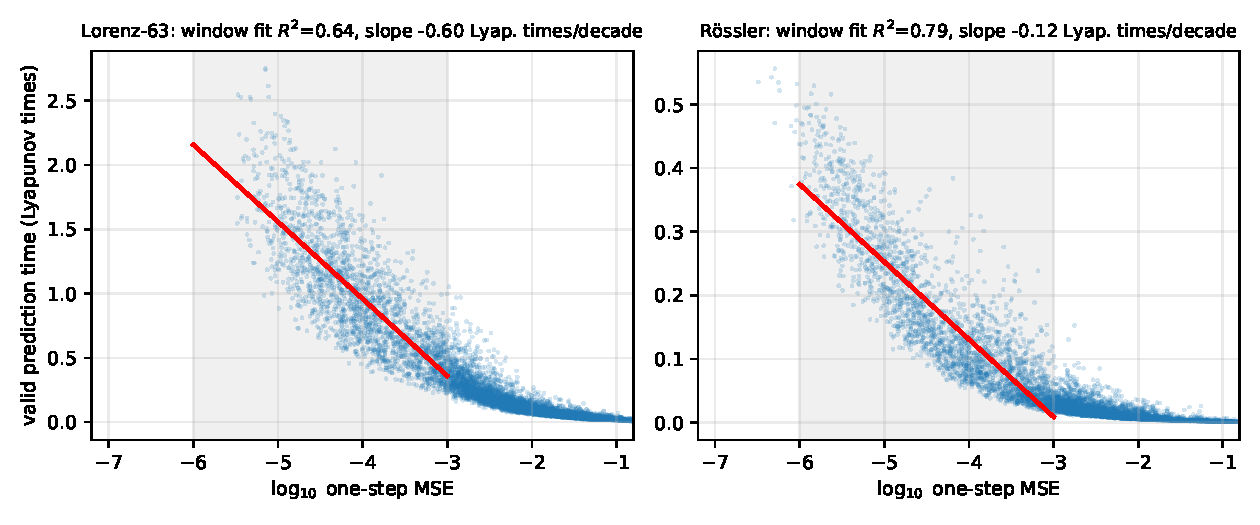
\includegraphics[width=0.95\textwidth]{figures/fig_vpt_law.pdf}
\caption{Valid prediction time versus one-step MSE for all models of valid parents; the shaded window is where the log-linear fit (red) is made.}\label{fig:law}
\end{figure}

\begin{table}[t]
\centering\scriptsize
\caption{Log-linear fit of VPT on $\ln\mathrm{MSE}$ under two selection rules. $\lambda_{\mathrm{eff}}=-1/(2\,\mathrm{slope})$ in inverse time units. Last column (window fit only): Spearman correlation across parents of per-parent $\lambda_{\mathrm{eff}}$ with the parent's Lyapunov exponent, tangent growth rate, and mean log largest singular value rate.}\label{tab:law}
\resizebox{\textwidth}{!}{%
\begin{tabular}{llccccccl}
\toprule
System & Selection & models & $R^2$ & per-parent $R^2$ & slope (Lyap.\ times/decade) & $\lambda_{\mathrm{eff}}$ & $\lambda_{\mathrm{eff}}/\lambda$ & $\rho$ (LLE, tangent, $\sigma_{\max}$)\\
\midrule
Lorenz-63 & $\log_{10}$MSE in $[-6,-3]$ & 2121 & 0.64 & 0.42--0.79 & -0.60 & 1.74 & 1.9 & -0.09, -0.15, +0.26 \\
Lorenz-63 & VPT $>0.05$ (sensitivity) & 6688 & 0.83 & -- & -0.43 & 2.44 & 2.7 & -- \\
R\"ossler & $\log_{10}$MSE in $[-6,-3]$ & 2668 & 0.79 & 0.75--0.85 & -0.12 & 0.62 & 9.4 & +0.08, -0.01, -0.05 \\
R\"ossler & VPT $>0.05$ (sensitivity) & 2206 & 0.72 & -- & -0.11 & 0.66 & 10.0 & --\\
\bottomrule
\end{tabular}}
\end{table}

\begin{table}[t]
\centering\small
\caption{Leave-one-parent-out $R^2$ for predicting VPT in the MSE window. The two parent-based models are evaluated only on parents whose rate exceeds $0.02$.}\label{tab:loo}
\begin{tabular}{lcc}
\toprule
Model & Lorenz-63 & R\"ossler\\
\midrule
Constant slope per system & 0.64 & 0.79 \\
Slope from parent Lyapunov exponent & 0.62 & 0.10 \\
Slope from parent Jacobian expansion rate & 0.33 & 0.19\\
\bottomrule
\end{tabular}
\end{table}

\subsection{Validity range of first-order Lyapunov response}
We checked $S_{lin}$ on a single Lorenz parent with 40 isotropic perturbations per norm. Against the \emph{exact} change in the orbit-averaged tangent growth rate along the same fixed orbit, $S_{lin}$ is accurate at relative norm $10^{-4}$ (correlation $0.998$, slope $0.99$) but degrades rapidly ($0.87$ at $10^{-3}$, $0.38$ at $3\times10^{-3}$, $0.03$ at $10^{-2}$), while the version without the direction term is uninformative at $10^{-4}$ (correlation $0.02$). Against the actual change in the LLE of the perturbed map on its own attractor, correlations are between $-0.08$ and $0.45$ and sign agreement is $0.47$--$0.55$; at $10^{-4}$ the estimator noise (standard deviation $8\times10^{-3}$) exceeds the first-order signal ($3\times10^{-3}$). Compression perturbations (relative norm $\ge0.007$ here, typically $0.1$--$0.6$) lie far outside this regime (Figure~\ref{fig:slin}).

\begin{figure}[t]
\centering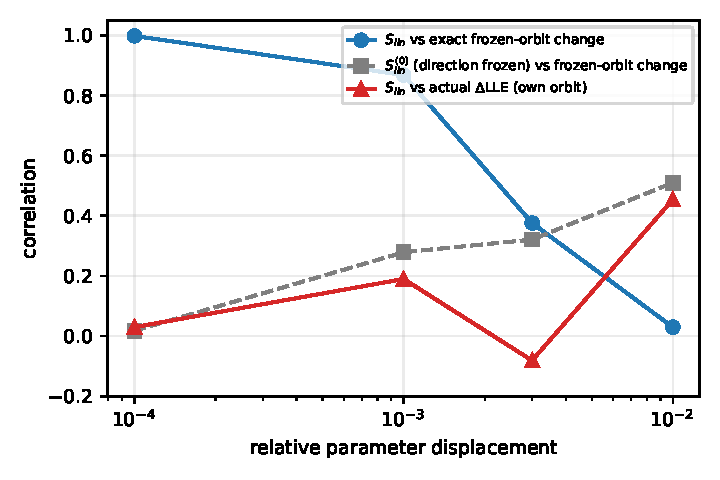
\includegraphics[width=0.55\textwidth]{figures/fig_slin_validity.pdf}
\caption{Correlation between first-order prediction and measured change versus perturbation size (one Lorenz parent, 40 draws per norm).}\label{fig:slin}
\end{figure}

\section{Discussion}
\paragraph{Does equal norm mean equal dynamics?} Not in failure behaviour and, modestly, not in predictive accuracy. At matched norm, structured perturbations are usually less damaging than isotropic noise by VPT and one-step error, and failure modes differ markedly (divergence for pruning, collapse for noise on Lorenz). However, the differences are small compared with the effect of the norm itself, and they largely vanish when per-tensor norms are matched. We therefore do not claim a universal ordering of perturbation families; for LLE the data are insufficient to make any claim, because most perturbed models fail.

\paragraph{One-step error and long-run behaviour.} The strong relationship between one-step error and VPT loss should not be over-read: it holds for short-horizon rollout accuracy of post-hoc perturbations. For the long-run exponent, one-step error has no predictive value on R\"ossler and modest value on Lorenz, so a low one-step error after compression does not certify a preserved attractor. The robustness radius makes the same point from the other side: half of isotropic perturbations of only a few percent of the parameter norm destroy the attractor, a scale reached by 6-bit quantization, so attractor survival, not accuracy, is the binding constraint for aggressive compression of such surrogates. This is consistent with the broader message of~\cite{liu2026sns,robertson2026} that local and long-horizon objectives differ, while our results add that, for a fixed network, local error tracks the short-horizon part well.

\paragraph{Is failure silent?} Mostly not. Almost every failed surrogate already has a markedly larger one-step error than its parent (98--99\%), so H1 is not supported as a general statement. Two qualifications apply. First, high one-step error does not single out failures, since about three quarters of survivors exceed the same threshold. Second, a minority of R\"ossler models, mostly at the smallest norms, diverge with near-parent one-step error, so low error does not certify survival there.

\paragraph{Jacobian measures.} The Jacobian-change measures improve on norm for VPT but did not beat one-step error, which is cheaper to compute. Their potential advantage lies in being label-free with respect to targets and in giving a direction-aware first-order theory; our evidence is that this theory is valid only for displacements far below those of compression and that the invariant-measure shift and orbit rearrangement dominate beyond it.

\section{Limitations}
\begin{itemize}
\item \textbf{Selection.} LLE and SW$_1$ analyses are conditional on a model surviving, which is 30\% (Lorenz) and 21\% (R\"ossler) of perturbed models, biased toward mild perturbations. VPT, MSE and failure comparisons are not conditional on survival.
\item \textbf{R\"ossler surrogates.} Eight of 30 parents were excluded and the remainder reproduce only about half of the reference exponent; R\"ossler LLE results should be considered uninformative.
\item \textbf{Scope.} Two three-dimensional systems, one small architecture, post-training compression only (no fine-tuning or quantization-aware training), one training recipe, and relative norms up to $0.6$.
\item \textbf{VPT is short-horizon.} Its strong association with one-step error is partly mechanical.
\item \textbf{Mechanism only partly tested.} The role of the output layer is supported by layer-matched controls and by displacement ratios, but the cross-validated check is weak (family adds nothing beyond norm) and no intervention perturbs a single tensor; the slope of the log-linear VPT relation is unexplained.
\item \textbf{Thresholds and functional forms.} The robustness radius depends on the collapse threshold and a logistic form; the VPT relation is fitted in a chosen MSE window ($R^2$ is lower on Lorenz, $0.64$) and is descriptive.
\item \textbf{Multiplicity.} Holm correction is applied within metric families; exploratory per-row $p$-values should be read as descriptive.
\item \textbf{H1 test.} It is post hoc and cross-sectional (Section~\ref{sec:h1}); the low-error failures are few (18 and 37 models) and concentrated in a minority of parents, so the R\"ossler exception should be treated as a lead rather than an established effect.
\item \textbf{Relation to the pilot.} The study is an independent re-implementation; differences from the preliminary pilot may reflect implementation and selection effects as well as sample size.
\end{itemize}

\section{Conclusions}
In a controlled study of 21{,}180 perturbed chaotic surrogates, the attractor survives only small parameter displacements, and failure is rarely silent (98--99\% of failed models already have at least ten times their parent's one-step error): half of isotropic perturbations destroy it at 4.4\% (Lorenz) and 1.8\% (R\"ossler) of the parameter norm, a scale reached by 6-bit quantization. At matched norm, structured perturbations differ from isotropic noise in failure mode and, modestly, in valid prediction time and one-step error, and most of this difference disappears when per-tensor norms are matched, with the small output layer the main place where isotropic noise and structured perturbations differ at matched total norm. Valid prediction time is approximately log-linear in one-step error in a window of moderate errors, with a system-specific slope that is not explained by Lyapunov or Jacobian statistics, and parent-relative one-step error adds substantial predictive power over norm for valid-prediction-time loss. Long-run exponent damage remains poorly predicted and, for most perturbed models, unmeasurable because they fail. Practically, compression of learned chaotic surrogates should be evaluated with failure rates and valid prediction time alongside any exponent estimate, and exponent comparisons should be reported together with the fraction of models that survive.

\section*{Data and code availability}
Code (NumPy implementation of training, perturbations, Lyapunov and valid-prediction-time estimators, sensitivity measures and analysis), configuration, per-model raw results for all 60 parents, and the scripts that generate every figure and table (including \texttt{analyze\_h1.py} for Section~\ref{sec:h1}) are archived on Zenodo at \href{https://doi.org/10.5281/zenodo.23157081}{doi:10.5281/zenodo.23157081}. The full experiment runs in about one hour on a single CPU core. All results were produced with fixed seeds $0$--$29$ per system.

\section*{Declarations}
\paragraph{Author contributions.} Single author: conceptualisation, methodology, software, formal analysis, writing.
\paragraph{Funding.} This research received no external funding.
\paragraph{Competing interests.} The author declares no competing interests.


\bibliographystyle{unsrtnat}
\bibliography{refs}

\appendix
\section{Configuration}
\begin{center}\small
\begin{tabular}{lp{0.74\textwidth}}
\toprule
Item & Setting\\
\midrule
Systems & Lorenz-63, R\"ossler; RK4, internal step $10^{-3}$, sampled at $0.02$, transient $20$\\
Data & 20{,}000 train and 5{,}000 test consecutive transitions per seed, standardised\\
Model & Residual MLP 3--64--64--3, tanh, Xavier init (output layer scaled $0.1$)\\
Training & Adam, lr $10^{-3}$, batch 128, 50 epochs, one-step MSE\\
Seeds & 30 per system (0--29)\\
Structured & global and layer-wise pruning $25/50/75\%$; quantization $8/6/4/3$ bit; random pruning $25/50/75\%$\\
Controls & isotropic, layer-matched, support-matched noise, 10 draws each; isotropic grid at $0.01,0.02,0.05,0.1,0.2,0.3,0.45,0.6$\\
LLE & 1{,}000 transient + 10{,}000 steps, analytic Jacobian, tangent renormalisation\\
Failure & divergence: $\|x\|_\infty>50$ or non-finite; collapse: state sd $<0.05$\\
VPT & 20 initial conditions, 500-step horizon, threshold $0.4$ on $\|\hat x-x\|/\sqrt3$\\
Usable LLE & not failed and half-run estimates within $0.25$\\
H1 analysis & parent-relative MSE bins ($<3$ to $>1000$); failure = diverged or collapsed; interval by bootstrap over parents (2{,}000)\\
Sensitivity orbit & parent's own 3{,}000-step orbit (true orbit if collapsed), burn-in 300\\
\bottomrule
\end{tabular}
\end{center}

\end{document}
